\documentclass[ENG,BIB]{TFUOC}%IB: CASTELLÀ, CAT: CATALÀ, ENG: ANGLISH

%Introduce Work Data
\title{TFM Integracion Multimodal de Transcriptomic Espacial}
\titcrt{} %Short title to appear in header
\author{Student: Marco Russo}
\date{September 21, 2026}


\nomPDC{Jose Francisco Sanchez-Herrero}
\nomPRA{David Merino Arranz}
\titulac{Master's degree in Bioinformatics and Biostatistics}
\area{Work Area: Omics Data Analysis}
\idioma{English}
\credits{15}
\parcla{Spatial Transcriptomics, Graph Attention Networks (GAT), Conditional Variational Autoencoder (C-mVAE), eXplainable AI (XAI), Biomarkers, Sex-stratified medicine.}

\licenc{ccBy}
%Possible licenses
%ccByNcNd
%ccByNcSa
%ccByNc
%ccByNd
%ccBySa
%ccBy
%GNU
%copyright


%%%%%%%%%%
% Summary in language

\abstractidioma{
Maximum 250 words, for the purpose, context of application, methodology, results and conclusions of the work.


}

% Summary in English.
\abstractenglish{
A maximum of 250 words, detailing the purpose, context of application, methodology, results and conclusions of the work. \\

This Master's Thesis (TFM) focuses on the field of Omics Data Analysis, specifically addressing the integration of spatial transcriptomics and single-cell RNA sequencing (scRNA-seq). The ultimate goal is to develop and implement a Deep Learning architecture combining Graph Neural Networks (GNN) and Multimodal Variational Autoencoders (VAE). This architecture will be explicitly conditioned by biological sex to model cellular heterogeneity in cardiovascular tissues. Upon completion, the project will deliver a trained model, an extraction of interpretable biomarkers using eXplainable Artificial Intelligence (XAI), and an interactive dashboard for visualization.
}

\begin{document}

\estructura

\tableofcontents

\listoffigures

\listoftables




\chapter{Introduction}

This Master's Thesis (TFM) focuses on the field of Omics Data Analysis, specifically addressing the integration of spatial transcriptomics and single-cell RNA sequencing (scRNA-seq). The ultimate goal is to develop and implement a Deep Learning architecture combining Graph Neural Networks (GNN) and Multimodal Variational Autoencoders (VAE). This architecture will be explicitly conditioned by biological sex to model cellular heterogeneity in cardiovascular tissues. Upon completion, the project will deliver a trained model, an extraction of interpretable biomarkers using eXplainable Artificial Intelligence (XAI), and an interactive dashboard for visualization.

\section{Context and justification of work}

Work starting point (What is the need to cover? Why is it a relevant issue? How is the problem solved at the moment?) and contribution made (What result do you want to obtain?).
It is important to bear in mind that the final work must be understandable for anyone who knows the area of knowledge, but does not have to be an expert in the subject of what the work is about.

***

Precision medicine requires understanding not only which genes are expressed but also the spatial and cellular context in which they do so. Historically, differences associated with biological sex in vascular diseases have been underrepresented in standard bioinformatics analyses, reducing the efficacy of treatments in women. This work justifies its relevance by proposing an algorithmic solution that does not treat biological sex merely as a confounding factor, but as a structural conditioning variable within the neural network, providing a significant methodological advancement in the research of specific biomarkers.


\section{Motivation}

The primary motivation stems from the desire to bridge over a decade of professional experience in Machine Learning and MLOps engineering with frontier challenges in bioinformatics and health data science. Academically, this Master's Thesis constitutes a fundamental pillar and an essential proof of concept in preparation for future Ph.D. studies in computational biology or bioinformatics, with a focus on biopharmaceutical applications.


\section{Work objectives}

\begin{itemize}
\item Design and train a Deep Learning architecture (GAT + C-mVAE) for spatial transcriptomics data.
\item Extract sex-specific ligand-receptor communication biomarkers using XAI techniques.
\item Deploy the results in an interactive web application that allows the exploration of cellular niches.
\item In scope: Use of public datasets (GEO), computational deconvolution, and predictive modeling.
\item Out of scope: Collection of in vivo or wet lab clinical samples, experimental clinical validation.
\end{itemize}


\subsection{Main Objective}

The explicit inclusion of biological sex as a conditioning variable in geometric and generative architectures significantly improves the identification and explainability of spatial cellular niches and transcriptomic biomarkers.

\subsection{Research Questions} 

\begin{enumerate}
\item How does the deconvolution of transcriptomic spots using a sex-disaggregated scRNA-seq atlas affect the quality of the initial spatial signal?
\item Is it possible to stabilize the joint training of GNNs and VAEs by introducing Feature-wise Linear Modulation (FiLM) layers conditioned by sex?
\item Which cellular communication axes (ligand-receptor) are prioritized by XAI algorithms in female versus male samples?
\end{enumerate}


\section{Focus and method followed}

\begin{description}
\item[Research strategy:] 
A quantitative and experimental research strategy will be adopted, evaluating algorithmic performance against baseline models (such as STAGATE) using established metrics (ARI, NMI).
\end{description}

\begin{description}
\item[Development methodology:] 
An iterative approach based on prototyping will be used, implementing reproducible Machine Learning operations (MLOps) pipelines.
\end{description}

\begin{description}
\item[Tools:] 
PyTorch Geometric (network architecture), Squidpy and Scanpy (spatial and scRNA-seq processing), GitHub (version control), Docker (isolated environments), and Streamlit or R Shiny (final dashboard creation).
\end{description}

\section{Impact on sustainability, ethics-social and diversity}
\label{s:etic}

The scientific core of this project is, by definition, the integration of the gender perspective and biological sex into precision medicine, seeking to correct the biases of generic models. Additionally:

\begin{enumerate}
\item SAGER (Sex and Gender Equity in Research) guidelines will be applied for the correct reporting of variables in the analyses.
\item All technical documentation and the final report will use inclusive and non-sexist language.
\item The visualization dashboard will be designed and tested to ensure that differences in results across various biological profiles are presented clearly and without presentation biases.
\end{enumerate}

\subsection{Identification of the SDGs}

\begin{description}
\item[SDG 3] 
(Good Health and Well-being): By advancing analytical techniques for precision medicine and the early identification of biomarkers in complex diseases.
\end{description}

\begin{description}
\item[SDG 5] 
(Gender Equality): By developing algorithms that correct historical biases in medical data through stratified and conditioned architectures.
\end{description}

\begin{description}
\item[SDG 9] 
(Industry, Innovation and Infrastructure): Providing technological innovation through the use of explainable artificial intelligence (XAI) in bioinformatics infrastructures..
\end{description}



\section{Work schedule}

Description of the necessary resources to do the work, the tasks to be carried out and a temporary planning of each task using a Gantt diagram or similar. This planning should mark the partial milestones of each of the CAPs.

\begin{figure}[htbp]
\begin{center}

\caption{default}
\label{default}
\end{center}
\end{figure}


\section{Brief summary of products obtained}

No need to go into detail: the detailed description will be made in the rest of the chapters.

%It is not necessary to enter in detail: the detailed description will be done in the rest of the chapters.

\section{Brief description of other memory chapters}

Brief explanation of the contents of each chapter and its relationship with the global project.

\chapter{PEC 2}

TBD

%\chapter{State of Art}

%State of the art of the subject in question. It should end up showing why work is important and contributes something, and with the hypotheses of work.


\chapter{Materials and methods}
In these sections, it is necessary to describe:
\begin{itemize}
    \item The most relevant aspects of the design and development of the work.
    \item The methodology chosen to carry out this development, describing the possible alternatives, the decisions taken, and the criteria used to make these decisions.
    \item The products obtained.
\end{itemize}

\chapter{Statement on the use of generative artificial intelligence}

Explanation of any use made of generative artificial intelligence tools (such as ChatGPT, Gemini, DALL-E, or others) during the conception and development of this Final Project, as well as the writing of this report and the preparation of the presentation. It is mandatory to specify the concrete tools used, the purpose (e.g., ideation, code outlining, grammatical correction, image generation, etc.), the periods or phases of the work in which they were employed, the actions taken to validate the content generated by AI, and a critical evaluation of the impact of their use. It must be explicitly clarified which parts of the work are entirely the student's authorship and which have been based on inputs or results generated by AI, ensuring at all times that the intellectual responsibility and final validation of the content fall entirely upon the student, and that its use has been discussed with the Project supervisor and carried out in accordance with their instructions.


 
\textbf{Chapter structuring may vary depending on the type of work.}  
 
If applicable, a section on “Economic evaluation of work” will be included. This section will indicate the expenses associated with the development and maintenance of work, as well as the economic benefits obtained and a final analysis on the viability of the product.



\chapter{Results}

Detail in this section the results obtained using the methodology described in the previous section.


%Recull of job results. There should be a correspondence with the methodology that the results are what is obtained after applying the methodology.

The figures must be explained and quoted in the text, such as \ref{fig:my_label}, in which the error is shown depending on the distance, in arbitrary units. All graphs must have the title of the axes.

\begin{figure}[!htbp]
    \centering
    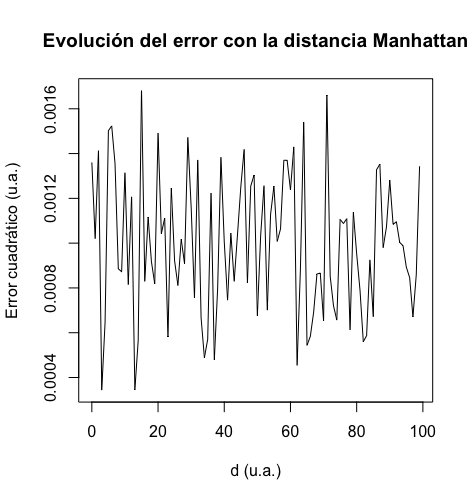
\includegraphics[width=7truecm]{Rplotmanh.png}
    \caption{Error working distance in arbitrary units.}
    \label{fig:my_label}
\end{figure}

%\chapter{Discussion}
%Discussion of results in project context. It is in this section that they make sense and in which the research questions are answered and it is shown how the results respond to the problems raised.

%This part may not apply depending on the type of work.

%\chapter{Economic evaluation}
%If applicable, a section of ``Economic evaluation of work' will be included. This section will indicate the expenses associated with the development and maintenance of work, as well as the economic benefits obtained. A final analysis on the viability of the product must be carried out.

\chapter{Conclusions and future works}

%\section{Conclusions}
This chapter must include:
\begin{itemize}
\item A description of the conclusions of the work:
\begin{itemize}
    \item Once the results have been obtained, what conclusions are drawn?
    \item Are these results as expected? Or have they been amazing? Why?
\end{itemize}
\item A critical reflection on the achievement of the objectives initially set:
\begin{itemize}
    \item Have we achieved all the objectives? If the answer is negative, why?
\end{itemize}
\item A critical analysis of the monitoring of planning and methodology throughout the product:
\begin{itemize}
    \item Has the schedule been followed?
    \item Has the planned methodology been adequate enough?
    \item Has it been necessary to introduce changes to ensure the success of the work? Why?
\end{itemize}
\item From the impacts foreseen in \ref{s:etic}, ethical-social, sustainability and diversity, evaluate/mention whether they have been mitigated (if they were negative) or whether they have been achieved (if they were positive). 
\item If unforeseen impacts have appeared in \ref{s:etic}, evaluate/mention how they have mitigated (if they were negative) or what they have contributed (if they were positive).
\item The future lines of work that have not been explored in this work and have remained pending.


%\item A description of the conclusions of the work: What lessons have been learned from work?
%\item A critical reflection on the achievement of the objectives initially set: Have we achieved all the objectives? If the answer is negative, why?
%\item Of the impacts foreseen in the section \ref{s:etic}, an assessment, or at least mention, of whether they have been mitigated (if they were negative) or whether they have been achieved (if they were positive). 
\end{itemize}

%\section{Future Lines}
%The future lines of work that could not be explored in this work and have been pending.

%\section{Schedule Tracking}
%A critical analysis of the monitoring of the planning and methodology throughout the work: 
%\begin{itemize}
%    \item  Have the schedule been followed? 
%    \item Has the planned methodology been adequate? 
%    \item Has it been necessary to introduce changes to ensure the success of the work? Why?
%\end{itemize}

\chapter{Glossary}

Definition of the most relevant terms and acronyms used in the Report.

%Defining the most relevant terms and acronyms used within the Memory.

\chapter{Bibliography}

Numbered list of bibliographic references used within memory. In each place where a reference is used within the text, it must be indicated by quoting the reference number, for example: [7].

It is very important to include all the references used and quote them appropriately, that is, including all the information necessary to identify the reference. The minimum information to be included according to the reference type is:

\begin{itemize}
\item Book: Authors, Title, Edition (if applicable) Editorial, City, Year.
\item  Journal article: Authors, Title, Name of the Journal, Home and End Page Number, Issue of the magazine / Volume, Year.
\item  Web: URL and date it was visited.
\end{itemize}

Information on how to quote documents: \url{http://biblioteca.uoc.edu/es/recursos/citacion-bibliografica}.


\newpage
\appendix
List of sections that are too extensive to include in memory and have a self-contained character (e.g. user manuals, installation manuals, etc.)
 
Depending on the type of work, there may be no need to add an annex.

\end{document}
